%%========================Introducao================================%%
\section{Dobramento de Proteínas}

%%========================Objetivo================================%%
\subsection{Proteínas}
\frame{
	\frametitle{Proteínas}
	
	\begin{block}{Proteínas}
		\begin{itemize}
			\item 	Estruturas compostas por uma ou mais cadeias de aminoácidos.
			\item 	Exercem um papel fundamental na natureza.
			\item   Responsáveis por muitas funções importantes da células vivas.
			\item 	São produtos de um processo chamado dobramento de proteínas.
			\item	Inicia a partir de uma cadeia de aminoácidos inicialmente desdobrada que será transformada em sua estrutura final/nativa.
		\end{itemize}
		
		
	\end{block}
}

\subsection{Problema de Dobramento Proteínas}
\frame{
	\frametitle{Problema de Dobramento de Proteínas}
	
	\begin{block}{Problema de Dobramento de Proteínas}
		\begin{itemize}
			\item Se preocupa em entender o processo de dobramento das proteínas.
			\item Também trata da predição da estruturas de proteínas.
			\item A predição das estruturas tem um amplo campo de aplicações:
			\begin{itemize}
				\item Síntese de novas proteínas e dobramentos.
				\item Síntese de novas drogas baseada nas estruturas.
				\item Obtenção de estruturas a partir de dados
				incompletos de ressonância magnética nuclear.
			\end{itemize}
			\item A determinação da estrutura nativa de proteínas é uma tarefa desafiadora até mesmo para modernos super computadores.
			\item Trata-se de um problema $NP$-Completo.
		\end{itemize}
	\end{block}
}


\subsection{Modelos de Representação de Proteínas}
\frame{
	\frametitle{Modelos de Representação de Proteínas}
	
	\begin{block}{Modelos de Representação de Proteínas}
		\begin{itemize}
			\item Diferentes modelos para representar proteínas existem.
			\item Modelos extremamente detalhados são computacionalmente caros.
			\item Modelos simplificados são largamente utilizados por pesquisadores por conta de sua simplicidade em representar as proteínas.
			\item Modelo Hidrofóbico-Polar (HP).
		\end{itemize}
		
		
	\end{block}
}


\subsection{Modelo Hidrofóbico-Polar}
\frame{
	\frametitle{Modelo Hidrofóbico-Polar}
	
	\begin{block}{Modelo Hidrofóbico-Polar}
		\begin{itemize}
			\item Generaliza os aminoácidos que compõem as proteínas em apenas dois aminoácidos: hidrofóbicos H ou polares P.
			\item Utiliza um \textit{grid} 2d ou um cubo 3d para representar as possíveis conformações de uma proteína.
			\item No modelo HP existem 3 interações entre os aminoácidos H-P, P-P e H-H.
			\item Para calcular a energia de uma conformação no modelo HP é necessário avaliar a quantidade interações hidrofóbicas (H-H) entre aminoácidos não consecutivos na sequência.
		\end{itemize}
	\end{block}
}

\subsection{Modelo Hidrofóbico-Polar}
\frame{
	\frametitle{Modelo Hidrofóbico-Polar}
	
	\begin{block}{Modelo Hidrofóbico-Polar}
		\begin{figure}[!htb]
			\centering
			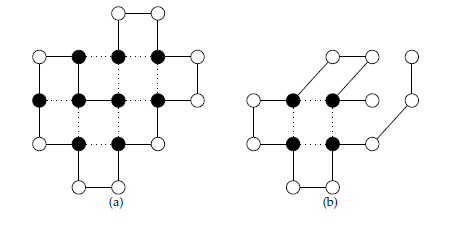
\includegraphics[scale=.8]{figuras/modeloHPExemplo.png}
			\caption{Exemplos de representação de proteínas utilizando os modelos HP 2D-HP (a) e 3D-HP (b). Fonte: Adaptado de }
			\label{fig:exemploModeloHP}
		\end{figure}
	\end{block}
}